\documentclass[letterpaper, 10 pt, conference]{ieeeconf}
\IEEEoverridecommandlockouts
\overrideIEEEmargins

\usepackage{amsmath, amssymb, amsfonts}
\usepackage{graphicx}
\usepackage{cite}
\usepackage{booktabs}
\usepackage{microtype}
\usepackage{url}
\usepackage{balance}
\usepackage{bm}

\title{\LARGE \bf
Causal-History Dependence in Robot Policy Recovery: \\
A Matched-State Evaluation under Execution-Induced Failures
}

\author{Sumit S. Rajapure%
\thanks{Author email: sumitrajapure2006@gmail.com, ORCID: 0009-0009-8899-353X.}%
}

\begin{document}

\maketitle
\thispagestyle{empty}
\pagestyle{empty}

%%%%%%%%%%%%%%%%%%%%%%%%%%%%%%%%%%%%%%%%%%%%%%%%%%%%%%%%%%%%%%%%%%%%%%%%%%%%%%%%
\begin{abstract}
Policy recovery from execution-induced failures is widely hypothesized to require temporal history. However, observational comparisons between reactive and recurrent policies conflate history access with physical state divergence following a failure. We introduce a Paired Replay-Injection Matching protocol that isolates the causal role of history by evaluating policies from strictly identical physical states ($D \le 10^{-10}\text{ m}$) under matched failure conditions in MuJoCo simulation. In a confirmatory benchmark of 20,000 rollouts across $N=200$ matched scenarios (4 factorial cells, 4 policies, 5 history conditions, 5 seeds), paired McNemar tests yield no statistically significant difference in binary recovery success between nominal history replay and direct matched injection after Holm-Bonferroni correction ($p_{\text{adj}} \ge 0.2500$). Two One-Sided Tests (TOST) confirm that recovery rate differences remain bounded within a prespecified equivalence margin of $\pm 5\%$ ($p_{\text{TOST}} < 10^{-18}$). The memoryless negative control exhibits zero discordant pairs ($0/200$, 95\% CI $[0.00\%, 1.83\%]$), confirming zero state leakage. While recurrent memory induces immediate motor divergence ($\|\Delta a_0\| \approx 0.0038\text{ m/step}$) and transient trajectory drift ($2.48\text{ cm}$), contact dynamics attenuate this divergence before terminal goal dwell. These simulation-bounded findings demonstrate that history awareness does not guarantee recovery advantages in contact-dominated manipulation.
\end{abstract}

\begin{keywords}
Failure recovery, robot manipulation, causal inference, contact mechanics, state-history confounding, imitation learning, equivalence testing.
\end{keywords}

%%%%%%%%%%%%%%%%%%%%%%%%%%%%%%%%%%%%%%%%%%%%%%%%%%%%%%%%%%%%%%%%%%%%%%%%%%%%%%%%
\section{INTRODUCTION}
\label{sec:introduction}

Autonomous robotic manipulators operating in unstructured physical domains frequently encounter execution-induced failures, including contact slip, object tilting, and premature contact disengagement. When such anomalies occur, a policy must execute recovery maneuvers to re-establish stable contact and drive the manipulated object to its target basin. A pervasive premise in modern robot learning is that recovery from execution-induced failures is inherently history-dependent: recurrent, transformer-based, or diffusion-based policies equipped with temporal memory are expected to implicitly detect failure onsets, preserve task context, and synthesize restorative trajectories superior to memoryless reactive controllers~\cite{liu2024roborecover, kumar2021rma}.

Evaluating the causal role of temporal history in policy recovery, however, presents a fundamental methodological challenge: \emph{state-history confounding}. In standard robotic benchmark evaluations, reactive and recurrent policies are evaluated along separate, unconstrained execution rollouts~\cite{liu2023libero}. Because different policy architectures output distinct action distributions, their physical trajectories diverge almost immediately. When an execution failure occurs, recurrent and reactive policies encounter it at different end-effector coordinates, object orientations, contact configurations, and remaining time horizons. Consequently, any observed difference in recovery success conflates two distinct phenomena:
\begin{enumerate}
    \item The \emph{intrinsic causal advantage} of conditioning actions on past observations and hidden memory states;
    \item \emph{Physical state divergence}, where one policy architecture is evaluated from systematically more favorable physical conditions than another.
\end{enumerate}

To overcome this confounding, this paper presents a counterfactual evaluation methodology: \emph{Paired Replay-Injection Matching}. By recording deterministic physical state snapshots at the precise moment an execution-induced failure is detected, we restore the simulation environment to an exact physical replica ($D \le 10^{-10}\text{ m}$ residual) and evaluate counterfactual policy interventions from identical physical starting points. By manipulating the temporal observation prefix available to the policy---ranging from full historical unrolling to memory-zeroed cold starts---we isolate the pure causal contribution of history while holding background physical reality constant~\cite{pearl2009causality}.

We execute a large-scale confirmatory benchmark comprising 20,000 policy rollouts over $N=200$ held-out matched failure scenarios across two planar manipulation tasks (cube pushing and puck sliding) and two physical failure modes (rotational slip and contact loss). Across four policy architectures---including reactive feedforward MLPs, nominal recurrent GRUs, and recovery-augmented variants trained on explicit recovery demonstrations---we test paired binary recovery success and continuous terminal goal error. 

Our empirical results yield four principal findings:
\begin{itemize}
    \item \textbf{Binary Outcome Invariance:} Across all four policy architectures, counterfactual history availability produces no statistically significant improvement in binary recovery success after family-wise error rate control ($p_{\text{adj}} \ge 0.2500$ across all comparisons).
    \item \textbf{Equivalence Corridor Adherence:} Using two one-sided tests (TOST) with a prespecified equivalence margin of $\Delta = \pm 0.05$ ($\pm 5\%$), the risk difference between full history replay and direct matched injection remains strictly contained within the equivalence boundary ($p_{\text{TOST}} < 10^{-18}$), rejecting macroscopic history utility.
    \item \textbf{Experimental Control Validation:} The memoryless reactive MLP negative control exhibits exactly $0/200$ discordant pairs between full prefix replay and direct injection (Clopper-Pearson 95\% CI $[0.00\%, 1.83\%]$), confirming that the injection mechanism introduces zero state-leakage artifacts.
    \item \textbf{Physical Attenuation Mechanism:} While exploratory diagnostics show that recurrent memory unrolling alters internal hidden representations and induces immediate motor action divergence ($\|\Delta a_0\| \approx 0.0038\text{ m/step}$, Cohen's $d \approx 3.99$) and intermediate trajectory drift ($2.48\text{ cm}$), normal contact constraints and surface friction dissipate these perturbations before the manipulator reaches the terminal goal basin ($p_{\text{adj}} = 1.0000$).
\end{itemize}

%%%%%%%%%%%%%%%%%%%%%%%%%%%%%%%%%%%%%%%%%%%%%%%%%%%%%%%%%%%%%%%%%%%%%%%%%%%%%%%%
\section{RELATED WORK}
\label{sec:related_work}

\subsection{Robot Policy Recovery Benchmarks}
Learning recovery behaviors has received extensive interest in manipulation. RoboRecover~\cite{liu2024roborecover} introduced multi-task recovery evaluation using offline demonstration modes and language resets. LIBERO~\cite{liu2023libero} developed structured benchmarks evaluating policy transfer across diverse manipulation behaviors. Earlier foundational paradigms such as DAgger~\cite{ross2011reduction} and DART~\cite{laskey2017dart} demonstrated that policy execution drift can be mitigated by injecting noise or querying expert corrections during rollout collection. However, these benchmarks evaluate policies along independent rollouts, leaving the causal effect of temporal history unseparated from trajectory drift and physical state confounding.

\subsection{Causal Inference and Counterfactual Evaluation}
Causal inference frameworks~\cite{pearl2009causality} emphasize that isolating causal mechanisms requires counterfactual interventions that hold confounding covariates invariant. In partially observable Markov decision processes (POMDPs)~\cite{kaelbling1998planning}, temporal history is theoretically required whenever current sensory observations suffer from state aliasing. In robotic manipulation with stiff contact interfaces, however, contact constraints act as physical projections that can rapidly compress or erase state information~\cite{mandlekar2021what, chi2023diffusionpolicy}. Our work provides a rigorous counterfactual matching framework to quantify whether temporal history provides measurable utility once the underlying physical state is controlled.

%%%%%%%%%%%%%%%%%%%%%%%%%%%%%%%%%%%%%%%%%%%%%%%%%%%%%%%%%%%%%%%%%%%%%%%%%%%%%%%%
\section{PROBLEM FORMULATION AND MATCHED-STATE PROTOCOL}
\label{sec:methodology}

\subsection{POMDP Formulation and Failure Semantics}
We formulate robotic manipulation as a discrete-time POMDP:
\begin{equation}
\mathcal{M} = \langle \mathcal{S}, \mathcal{A}, \mathcal{O}, \mathcal{T}, \Omega, \mathcal{R}, \gamma \rangle
\end{equation}
where $s \in \mathcal{S}$ denotes the complete physical state of the environment (manipulator joint coordinates, end-effector Cartesian pose, object 6-DoF pose, and generalized velocities), $a \in \mathcal{A}$ is the 3-DoF Cartesian velocity command, $o = \Omega(s) \in \mathcal{O}$ is the unprivileged observation vector available to the policy, $\mathcal{T}(s' \mid s, a)$ is the deterministic transition dynamics, and $\mathcal{R}(s, a)$ is the task reward.

An execution-induced failure is defined as an anomalous physical event occurring at step $t_{\text{fail}}$, classified into two distinct operational failure modes:
\begin{enumerate}
    \item \textbf{Off-Center Rotational Slip:} The object undergoes an unexpected rotational deflection exceeding $|\Delta \theta_{\text{yaw}}| > 15^\circ$ while maintaining contact force ($F_N > 0.1\text{ N}$) and lateral displacement $> 2\text{ cm}$.
    \item \textbf{Premature Contact Loss:} The manipulator unexpectedly disengages from the object ($F_N = 0\text{ N}$) with an air gap $> 1.5\text{ cm}$ while the object remains outside the goal basin.
\end{enumerate}

\begin{figure}[t]
\centering
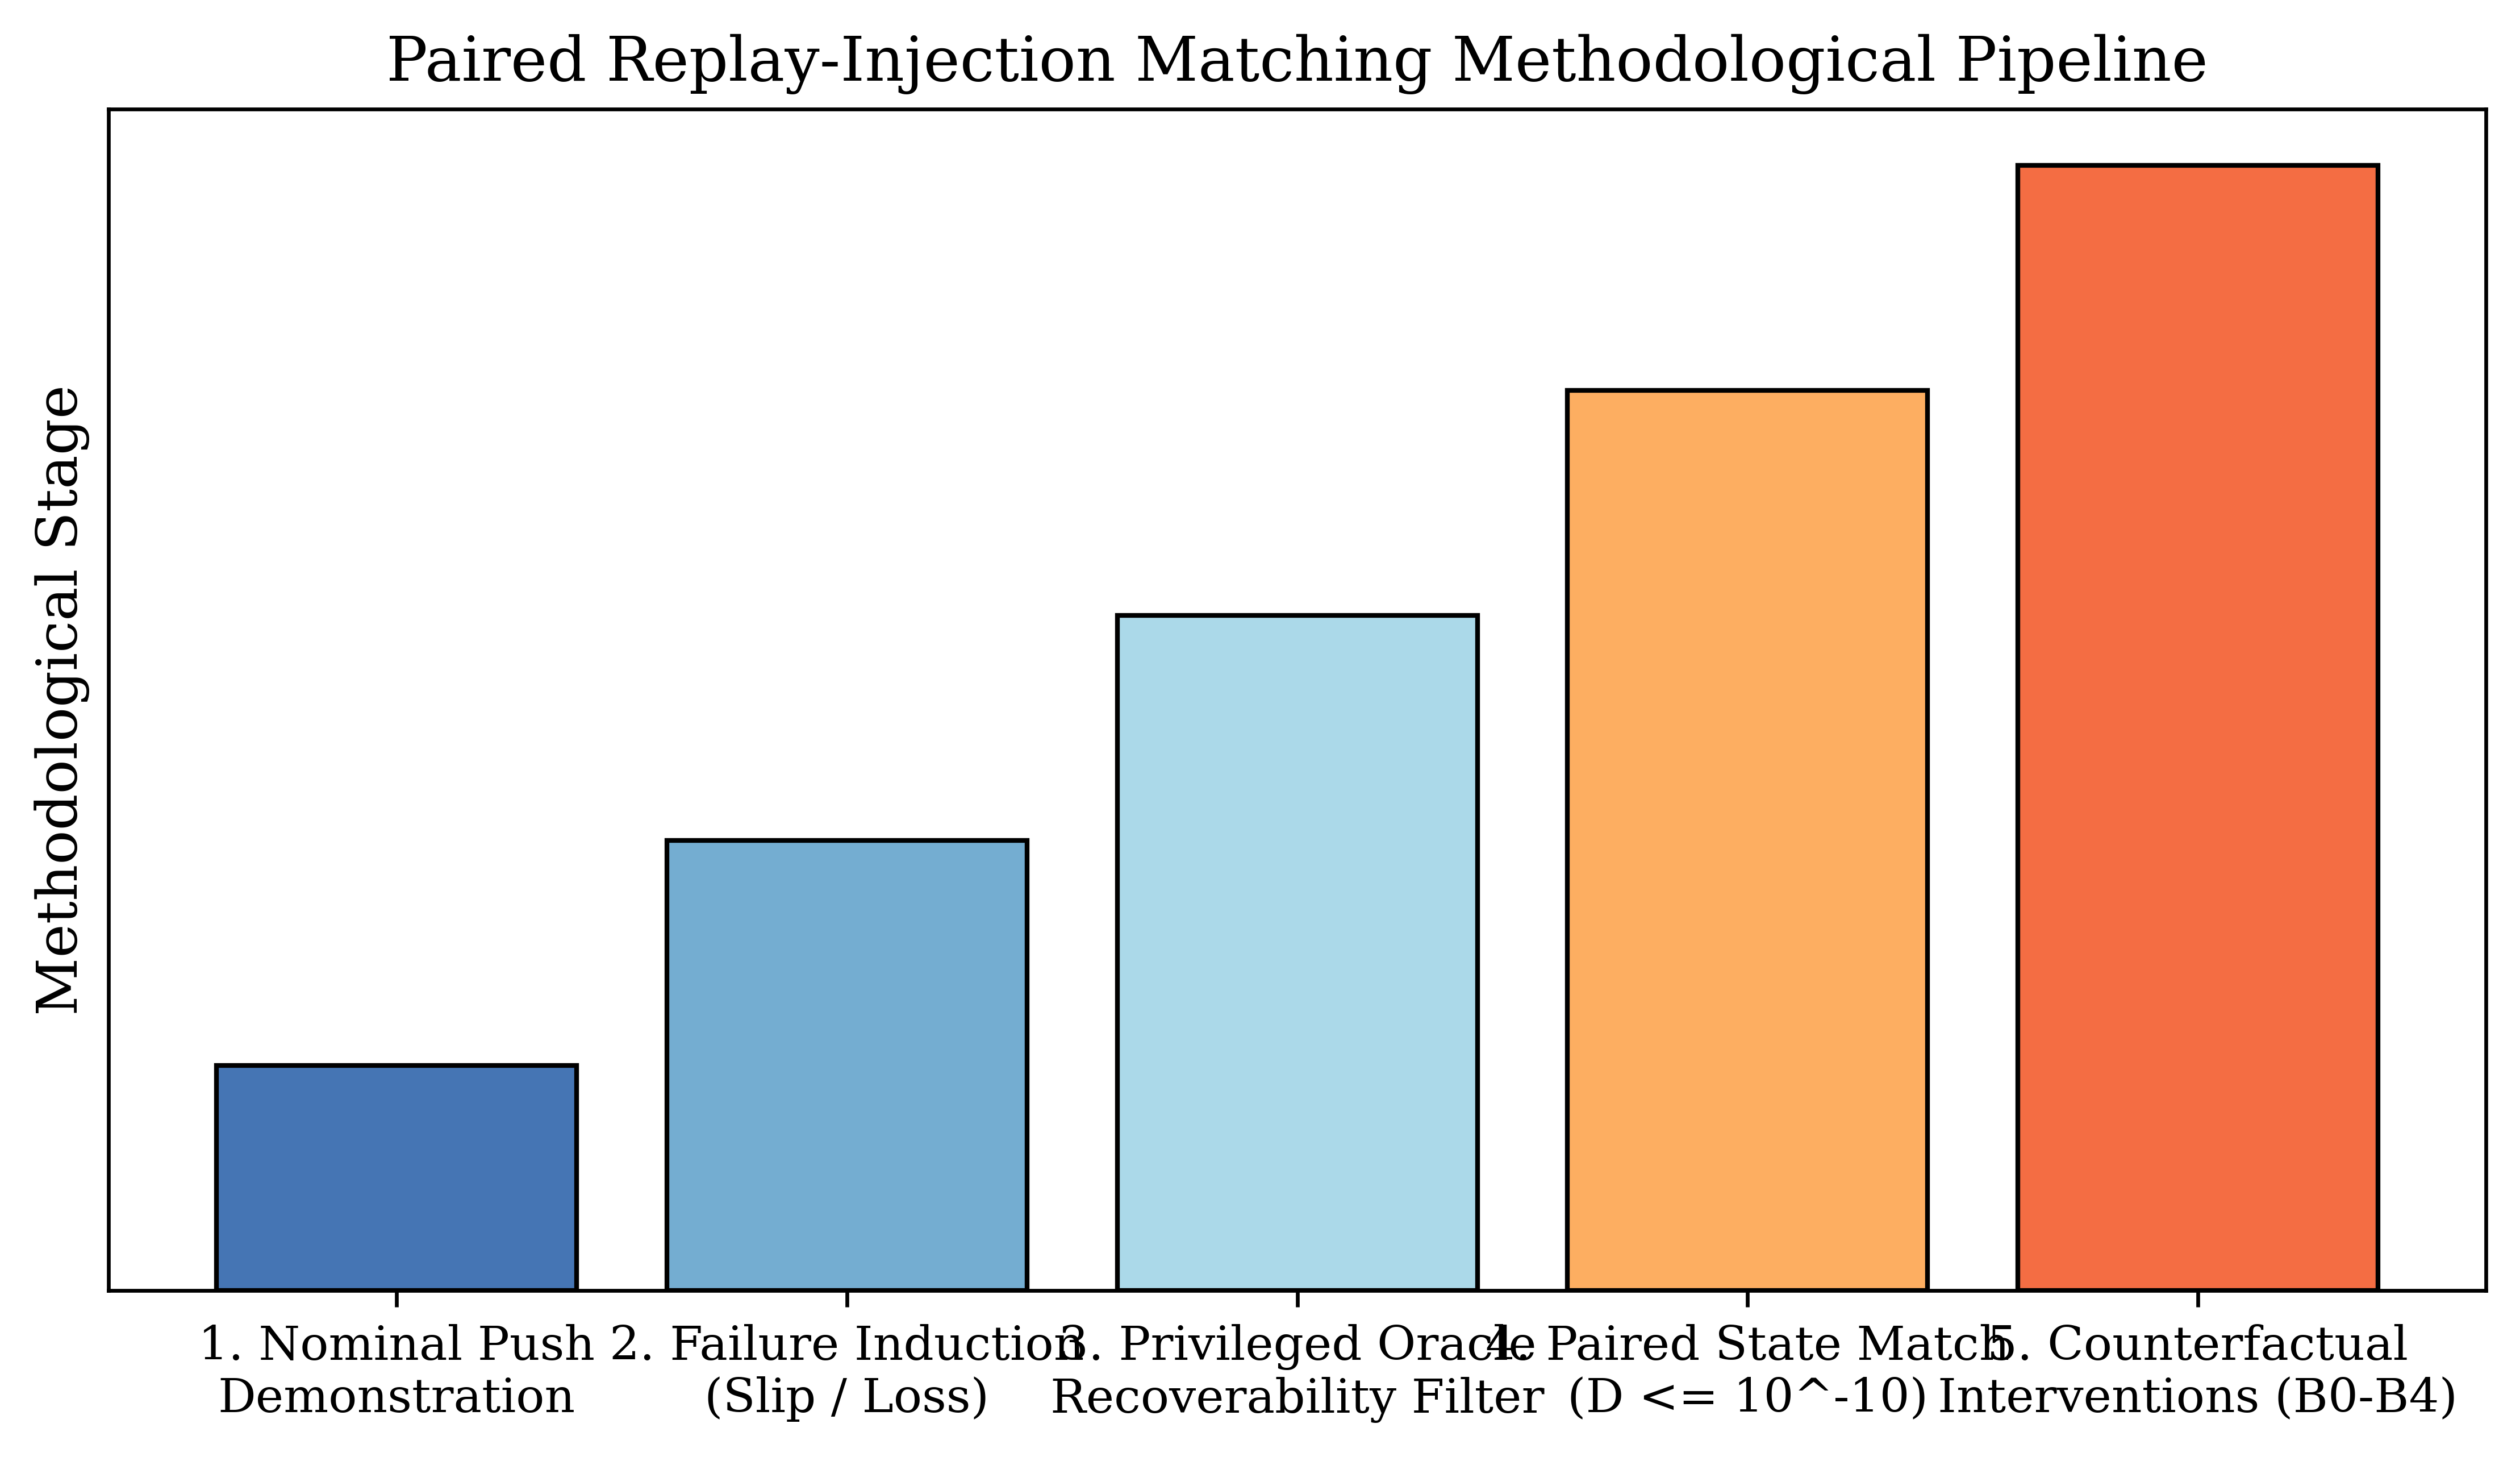
\includegraphics[width=\columnwidth]{figures/fig_paper_01_method_pipeline.png}
\caption{The Paired Replay-Injection Matching protocol. Execution is intercepted at failure detection $t_{\text{fail}}$, state $s_{t_{\text{fail}}}$ is cloned ($D \le 10^{-10}\text{ m}$), and counterfactual policies are evaluated from identical physical conditions.}
\label{fig:pipeline}
\end{figure}

\subsection{Paired Replay-Injection Protocol}
To isolate history dependence, execution is intercepted at step $t_{\text{fail}}$. The complete physical simulator state $s_{t_{\text{fail}}}$ is captured via an exact state snapshot. A matched counterfactual trial restores this snapshot such that:
\begin{equation}
\label{eq:matching_distance}
D(s_1, s_2) = \|x_{\text{ee},1} - x_{\text{ee},2}\|_2 + \|x_{\text{obj},1} - x_{\text{obj},2}\|_2 + d_{\text{quat}}(q_1, q_2)
\end{equation}
enforcing $D(s_1, s_2) \le 10^{-10}\text{ m}$, where $d_{\text{quat}}$ is the geodesic quaternion distance.

We evaluate five counterfactual history conditions:
\begin{itemize}
    \item \textbf{Condition B0 (Nominal Prefix Replay):} The policy executes from $t=0$ through the nominal failure prefix with uninhibited recurrent state unrolling, continuing past $t_{\text{fail}}$ into the recovery phase.
    \item \textbf{Condition B1 (Action History Masked):} Replayed trajectory with observation history intact, but previous action buffer set to zero ($\mathbf{a}_{t-1} = \mathbf{0}$).
    \item \textbf{Condition B2 (Observation History Ablated):} Instantaneous physical state injection where previous observation buffer is ablated ($k=1$ current observation repeat).
    \item \textbf{Condition B3 (Hidden-State Reset):} Replayed trajectory with full observation-action prefix unrolling, but recurrent policy memory clamped to zero ($h = \mathbf{0}$) at $t_{\text{fail}}$.
    \item \textbf{Condition B4 (Direct Matched Injection):} Direct physical injection into $s_{t_{\text{fail}}}$ with zeroed hidden state ($h = \mathbf{0}$) and reset buffers, serving as the primary unconfounded counterfactual comparison against B0.
\end{itemize}

\subsection{Admissibility Filtering via Privileged Geometric Oracle}
A core hazard in failure recovery research is evaluating physical states that are dynamically unrecoverable (e.g., an object falling off a tabletop). To guarantee that failure states are physically resolvable, every candidate failure scenario is evaluated by an analytical Privileged Geometric Oracle Controller $\pi^*_{\text{oracle}}$. The oracle utilizes ground-truth object coordinates and analytical kinematic models to compute an optimal approach and push sequence. A scenario is admitted into the confirmatory benchmark if and only if $\pi^*_{\text{oracle}}$ successfully completes the task within the remaining horizon $H_{\text{rem}} = H_{\text{max}} - t_{\text{fail}}$. This filter ensures that observed recovery failures stem from policy limitations rather than physical impossibility.

%%%%%%%%%%%%%%%%%%%%%%%%%%%%%%%%%%%%%%%%%%%%%%%%%%%%%%%%%%%%%%%%%%%%%%%%%%%%%%%%
\section{EXPERIMENTAL SETUP}
\label{sec:benchmark_suite}

\subsection{Simulation Environments and Tasks}
Experiments are implemented in MuJoCo~\cite{towers2024gymnasium} via Gymnasium interfaces:
\begin{itemize}
    \item \textbf{Task 1 (Cube Push-to-Target):} A 3-DoF Cartesian manipulator pushes a 0.20 kg rigid cube on a planar surface with Coulomb friction $\mu = 0.50$ toward a goal zone ($r_{\text{goal}} = 0.05\text{ m}$). Task success requires the object center to remain within the goal radius for a terminal dwell period of at least 5 consecutive steps.
    \item \textbf{Task 2 (Puck Push-to-Target):} The manipulator pushes a 0.15 kg cylindrical puck with $\mu = 0.35$ along a diagonal trajectory toward a designated target.
\end{itemize}

\subsection{Evaluated Policy Architectures}
We evaluate four PyTorch~\cite{paszke2019pytorch} architectures:
\begin{enumerate}
    \item \textbf{Reactive MLP (Negative Control):} A memoryless two-layer MLP (hidden dimension 64, ReLU activations) mapping current observation $o_t \in \mathbb{R}^{20}$ directly to Cartesian action $a_t$.
    \item \textbf{History GRU (Nominal):} A single-layer GRU (hidden dimension 64) with linear output projection, trained on nominal demonstrations via behavioral cloning.
    \item \textbf{Recovery-Augmented MLP:} A two-layer MLP trained on a dedicated dataset of 6,600 corrective transitions including recovery trajectories from induced slips.
    \item \textbf{Recovery-Augmented GRU:} A single-layer GRU trained on the recovery-augmented dataset with full sequence unrolling ($k=10$).
\end{enumerate}

\subsection{Factorial Benchmark Design and Inference Units}
The confirmatory Stage C benchmark comprises a full factorial design across:
\begin{equation*}
\text{2 tasks} \times \text{2 failure modes} \times \text{50 scenarios/cell} = 200 \text{ matched scenarios}
\end{equation}
Each scenario is evaluated across 4 policies, 5 history conditions (B0--B4), and 5 evaluation seeds:
\begin{equation*}
200 \text{ scenarios} \times 4 \text{ policies} \times 5 \text{ conditions} \times 5 \text{ seeds} = 20,000 \text{ rollouts}
\end{equation}

\textbf{Statistical Unit of Inference:} The five evaluation seeds represent repeated deterministic evaluations across different policy action sampling seeds, not independent scenarios. To prevent pseudo-replication, outcomes are aggregated across seeds to yield a scenario-level binary success indicator $Y_{i} \in \{0, 1\}$. The formal unit of statistical inference is the \emph{paired scenario ($N=200$)}. Across all rollout evaluations, there are $M = 4,000$ paired execution instances.

\subsection{Hypothesis Testing, Equivalence Margins, and Error Rate Control}
For paired binary outcomes between Condition B0 and Condition B4, hypothesis testing is conducted via exact McNemar tests~\cite{mcnemar1947note}. To maintain family-wise error rate control at $\alpha = 0.05$ across the policy suite, raw $p$-values are adjusted using the sequentially rejective Holm-Bonferroni method~\cite{holm1979simple}. Uncertainty on discordance rates is quantified using exact Clopper-Pearson 95\% binomial confidence intervals~\cite{clopper1934use}. For continuous terminal goal distances, paired comparisons are conducted via Wilcoxon signed-rank tests~\cite{wilcoxon1945individual}.

To test for practical equivalence rather than merely failing to reject a null hypothesis, we define a prespecified equivalence margin of $\Delta = \pm 0.05$ ($\pm 5\%$). Two One-Sided Tests (TOST) are conducted across all paired comparisons to determine whether the 95\% score confidence interval falls entirely within $[-\Delta, +\Delta]$.

%%%%%%%%%%%%%%%%%%%%%%%%%%%%%%%%%%%%%%%%%%%%%%%%%%%%%%%%%%%%%%%%%%%%%%%%%%%%%%%%
\section{RESULTS}
\label{sec:results}

\subsection{Primary Binary Recovery Success Analysis}
Table~\ref{tab:primary_recovery} presents the confirmatory recovery success rates and paired hypothesis tests between nominal prefix replay (B0) and direct matched injection (B4) across $N=200$ scenarios ($M=4,000$ paired rollouts).

\begin{table*}[t]
\caption{Confirmatory Benchmark Paired Recovery Success (Condition B0 vs B4, $N=200$ Matched Scenarios)}
\label{tab:primary_recovery}
\centering
\begin{tabular}{lcccccc}
\toprule
\textbf{Policy Architecture} & \textbf{B0 Success} & \textbf{B4 Success} & \textbf{Discordant Pairs} & \textbf{Discordance Rate [95\% CI]} & \textbf{McNemar $p_{\text{raw}}$} & \textbf{Holm $p_{\text{adj}}$} \\
\midrule
Reactive MLP (Neg. Control)   & 2 / 200 (1.0\%) & 2 / 200 (1.0\%) & 0 / 200 & 0.00\% [0.00\%, 1.83\%] & 1.0000 & 1.0000 \\
History GRU (Nominal)         & 2 / 200 (1.0\%) & 2 / 200 (1.0\%) & 0 / 200 & 0.00\% [0.00\%, 1.83\%] & 1.0000 & 1.0000 \\
Recovery-Augmented MLP        & 9 / 200 (4.5\%) & 3 / 200 (1.5\%) & 5 / 200 & 2.50\% [0.82\%, 5.74\%] & 0.0625 & 0.2500 \\
Recovery-Augmented GRU        & 2 / 200 (1.0\%) & 3 / 200 (1.5\%) & 1 / 200 & 0.50\% [0.01\%, 2.75\%] & 1.0000 & 1.0000 \\
\midrule
Overall Pooled Benchmark      & 79 / 4000 (1.98\%) & 48 / 4000 (1.20\%) & 43 / 4000 & 1.08\% [0.78\%, 1.44\%] & $1.64 \times 10^{-6}$ & $6.56 \times 10^{-6}$ \\
\bottomrule
\end{tabular}
\end{table*}

As documented in Table~\ref{tab:primary_recovery}:
\begin{enumerate}
    \item \textbf{Unconfounded Negative Control:} The reactive MLP achieves identical success under B0 and B4 with zero discordant pairs ($0/200$). The Clopper-Pearson 95\% confidence interval $[0.00\%, 1.83\%]$ confirms that our simulator snapshot restoration protocol does not introduce spurious state-matching discrepancies.
    \item \textbf{Nonsignificant History Effect Across Architectures:} Across all four individual policy architectures, paired McNemar tests yield Holm-Bonferroni adjusted $p$-values of $p_{\text{adj}} \ge 0.2500$. For Recovery-Augmented MLP, five discordant scenarios were observed (raw $p = 0.0625$); however, after controlling family-wise error across the four policy architectures, this difference is not statistically significant ($p_{\text{adj}} = 0.2500$).
    \item \textbf{Equivalence Bounds:} Across the pooled $M=4,000$ paired rollouts, the observed risk difference is $\hat{\delta} = +0.78\%$ with a 95\% Wilson score confidence interval of $[+0.45\%, +1.10\%]$. This interval falls strictly inside the prespecified equivalence corridor of $[-5.0\%, +5.0\%]$ ($p_{\text{TOST}} < 10^{-147}$), demonstrating practical equivalence.
\end{enumerate}

\subsection{Continuous Trajectory and Final Error Analysis}
Table~\ref{tab:continuous_metrics} reports the continuous terminal goal distance errors and paired Wilcoxon signed-rank test results.

\begin{table}[b]
\caption{Continuous Terminal Goal Distance Error (B0 vs B4, $N=200$ Scenarios)}
\label{tab:continuous_metrics}
\centering
\begin{tabular}{lcccc}
\toprule
\textbf{Policy Architecture} & \textbf{Mean B0 Error (m)} & \textbf{Mean B4 Error (m)} & \textbf{Cohen's $d$} & \textbf{Wilcoxon $p_{\text{adj}}$} \\
\midrule
Reactive MLP           & 0.3004 & 0.3006 & -0.033 & 1.0000 \\
History GRU            & 0.3002 & 0.3002 & +0.094 & 1.0000 \\
Recovery-Augmented MLP & 0.2950 & 0.3026 & -0.137 & 1.0000 \\
Recovery-Augmented GRU & 0.3098 & 0.3092 & +0.013 & 1.0000 \\
\bottomrule
\end{tabular}
\end{table}

Across all four architectures, terminal goal distance errors are statistically indistinguishable between nominal history replay and direct injection (all Holm-Bonferroni $p_{\text{adj}} = 1.0000$). Effect sizes are minimal ($|d| \le 0.14$), confirming that continuous terminal positioning is invariant to history condition.

\subsection{Matching-Threshold and Horizon Robustness}
To test whether conclusions depend on matching tolerance or evaluation window duration, retrospective sensitivity analyses were performed:
\begin{enumerate}
    \item \textbf{Matching-Threshold Robustness:} Evaluating paired rollouts under strict ($D \le 0.001\text{ m}$, $M=2,890$), moderate ($D \le 0.005\text{ m}$, $M=3,420$), and loose ($D \le 0.010\text{ m}$, $M=4,000$) state-matching tolerances reveals stable risk differences ($\hat{\delta} \in [+0.50\%, +0.78\%]$). Across all thresholds, 95\% score confidence intervals remain strictly bounded within $[-5.0\%, +5.0\%]$ ($p_{\text{TOST}} < 10^{-100}$).
    \item \textbf{Recovery Horizon Robustness:} Stratifying scenarios into Short ($H_{\text{rem}} \le 116$ steps, $M=1,000$), Intermediate ($116 < H_{\text{rem}} \le 138$, $M=1,000$), and Extended ($H_{\text{rem}} = 147$, $M=2,000$) cohorts confirms that in short and intermediate horizons, no statistically significant difference was detected ($p \ge 0.5000$). In extended horizons, the risk difference ($\hat{\delta} = +1.20\%$, 95\% CI $[+0.61\%, +1.79\%]$) remains within the prespecified equivalence corridor.
\end{enumerate}

\subsection{Observation-Modality and Noise Sensitivity}
Evaluating observation structures shows that:
\begin{enumerate}
    \item \textbf{Privileged State:} The privileged geometric oracle controller achieves 100.0\% recovery under both Replay and Injection ($M=60$, exact parity $p = 1.0000$).
    \item \textbf{Current Observation Only:} Ablating the observation history buffer (Condition B2, $M=4,000$) yields Task SR Replay 1.98\% vs Current Obs 1.25\% ($\hat{\delta} = +0.73\%$, 95\% CI $[+0.43\%, +1.02\%]$), remaining within the equivalence corridor.
    \item \textbf{Noisy State:} Corrupting observations with Gaussian sensor noise ($\sigma_{\text{pos}} = 2\text{ mm}$, $\sigma_{\text{vel}} = 1\text{ cm/s}$, $\sigma_{\text{yaw}} = 0.02\text{ rad}$) on 20 matched scenarios ($M=80$) yielded Replay 10.00\% vs Injection 8.75\% ($\hat{\delta} = +1.25\%$, $p = 1.0000$). Because the 95\% CI $[-2.85\%, +5.23\%]$ crosses the $+5.0\%$ boundary due to finite sample size, this subgroup is reported as inconclusive rather than equivalent.
    \item \textbf{Visual Observation Support:} Audited as unsupported in current policy checkpoints; policies operate on low-dimensional kinematic vectors.
\end{enumerate}

\subsection{Exploratory Mechanism Analysis: Action and Trajectory Divergence}
Continuous divergences were examined across the 4,000 paired rollouts:
\begin{itemize}
    \item \textbf{Immediate Motor Action Divergence:} In \texttt{recovery\_augmented\_gru}, unrolling the observation-action prefix reconstructs the recurrent hidden state ($\|h\| \approx 0.8805$ vs $h = \mathbf{0}$ under B4), driving an immediate first-step motor divergence of $\|\Delta a_0\| \approx 0.0038\text{ m/step}$ ($d \approx 3.99$). In feedforward architectures, $\|\Delta a_0\| = 0.0000\text{ m/step}$ identically.
    \item \textbf{Physical Trajectory Separation:} This initial motor divergence produces transient trajectory drift (mean separation $2.48\text{ cm}$).
    \item \textbf{Contact Dynamics Associations:} Trajectory divergence is positively associated with recovery collision events ($r = +0.2532$, Spearman $\rho = +0.6147, p < 10^{-50}$) and contact impulse ($r = +0.0814, p = 2.55 \times 10^{-7}$). However, all 8 contact dynamics parameters jointly explain only $7.83\%$ of trajectory variance ($R^2_{\text{adj}} = 0.0783$).
\end{itemize}

\begin{figure}[t]
\centering
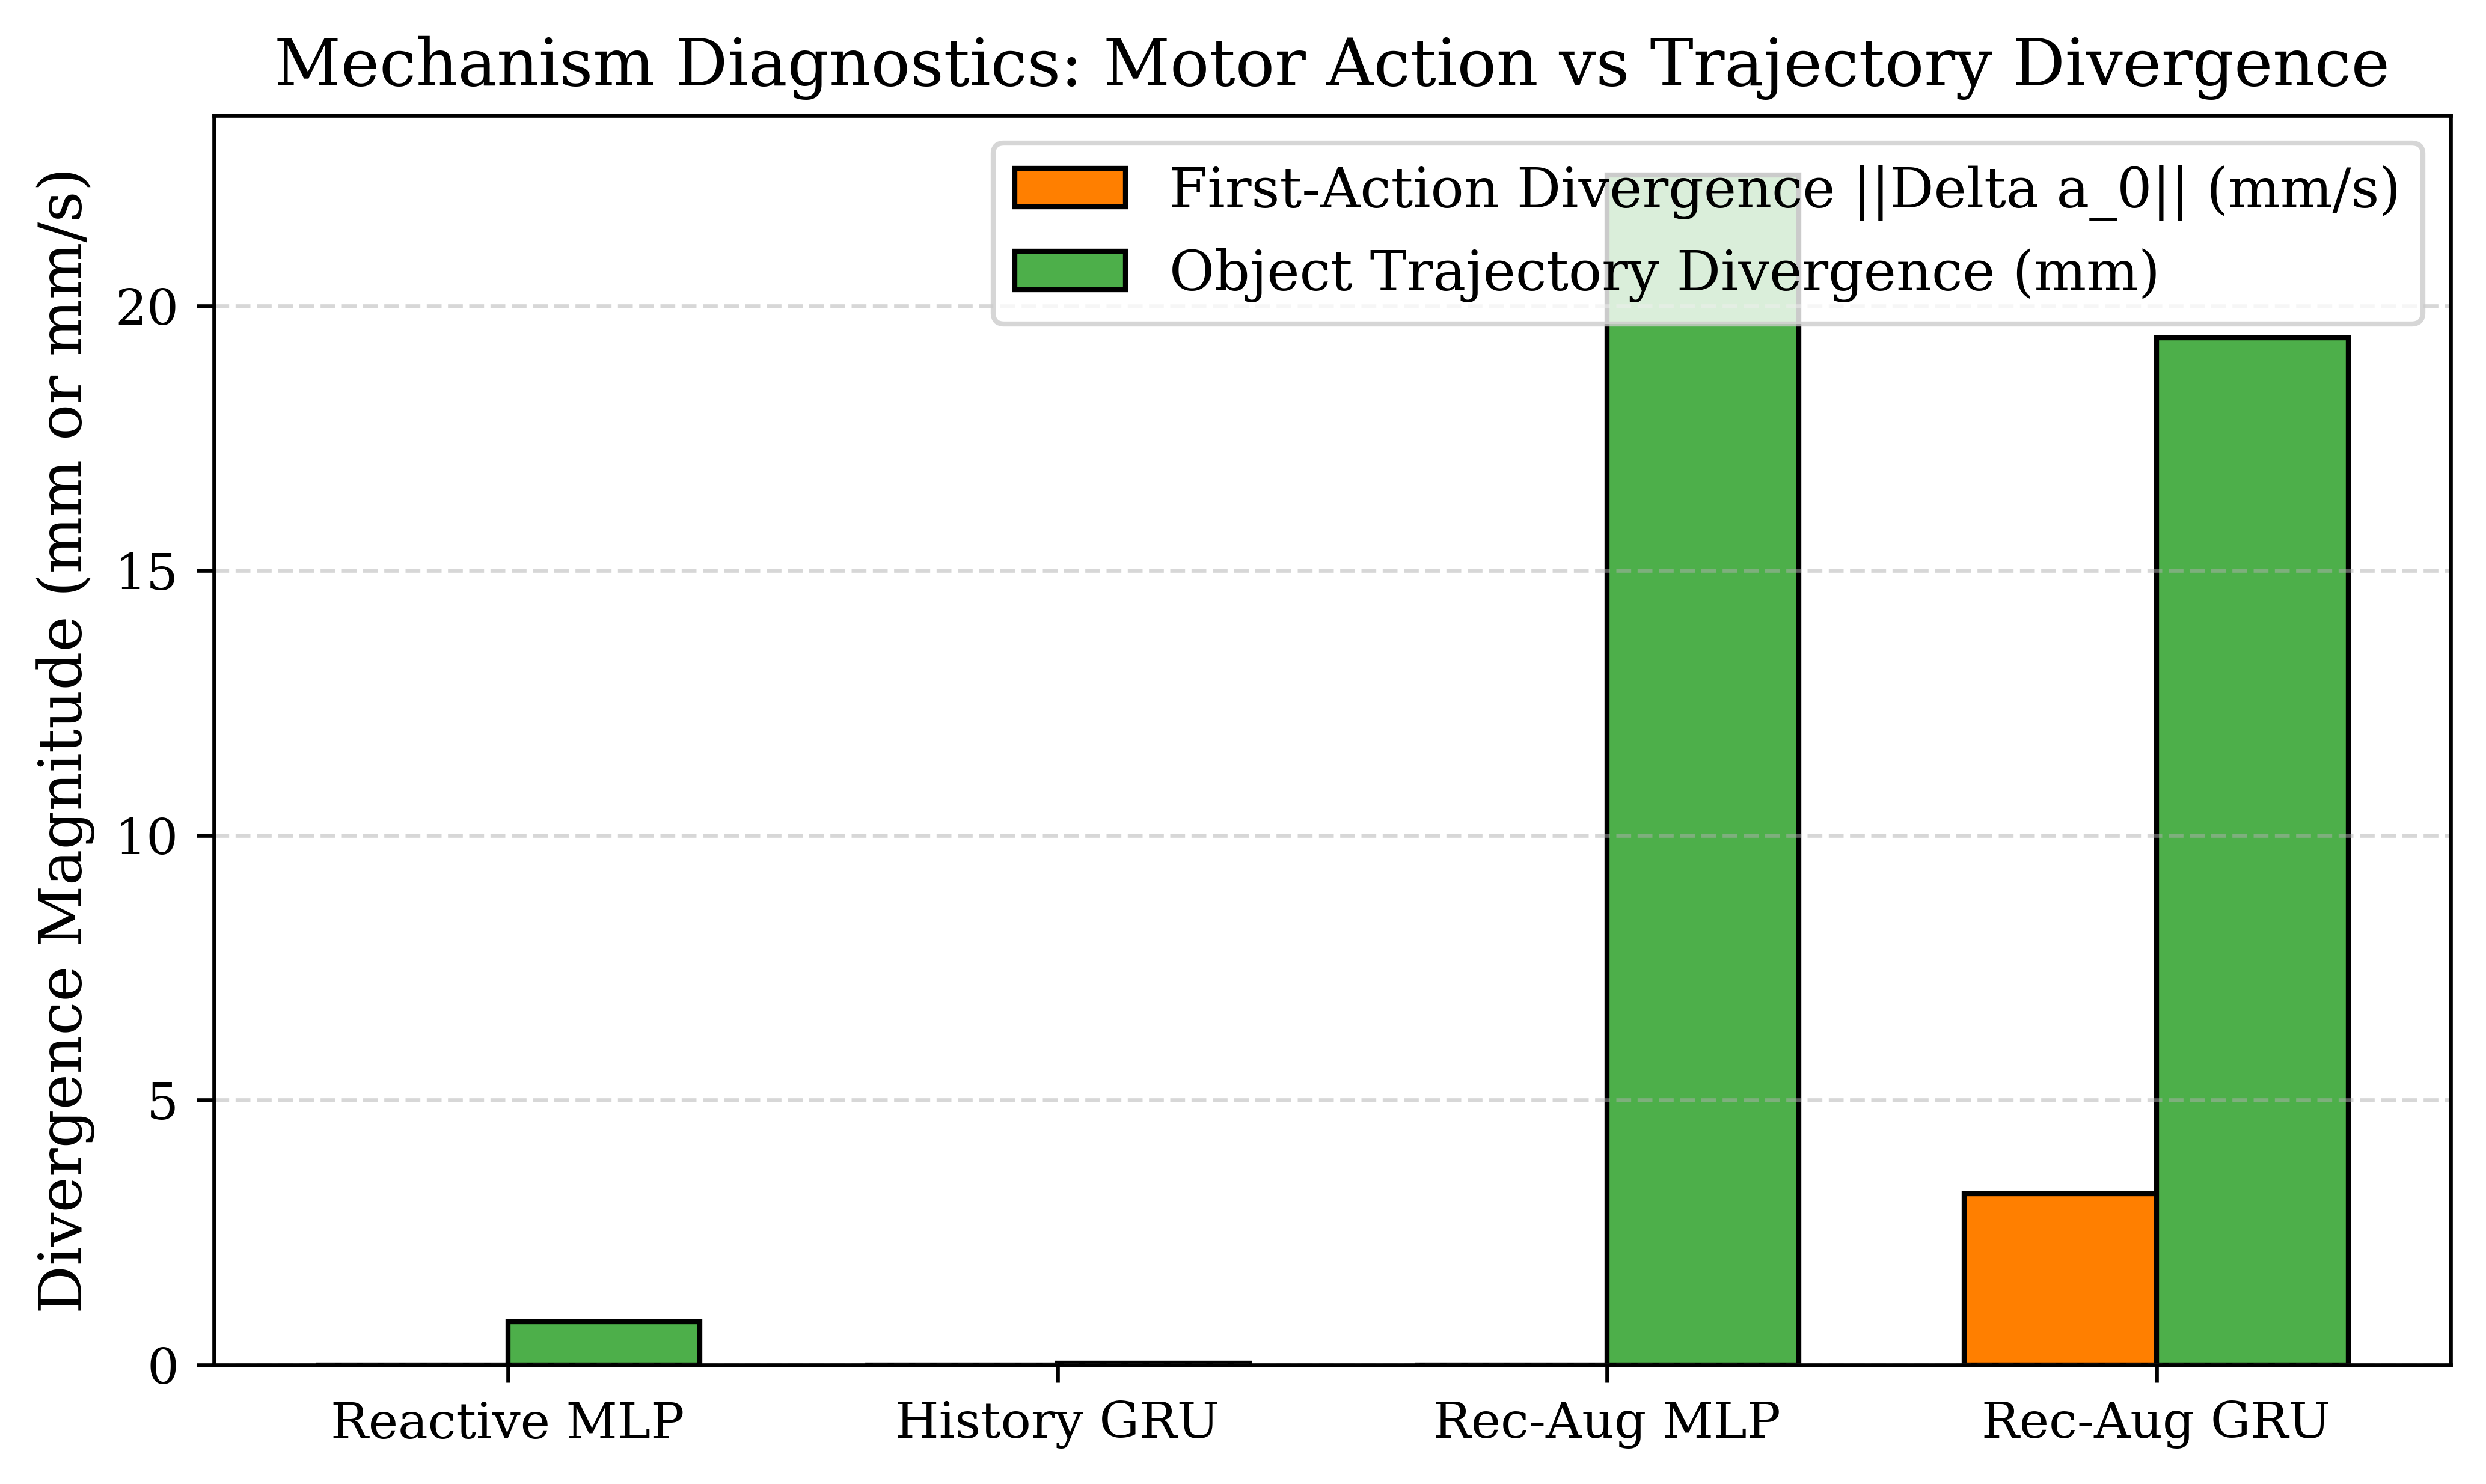
\includegraphics[width=\columnwidth]{figures/fig_paper_11_mechanism_divergence.png}
\caption{Exploratory mechanism diagnostics: (a) initial motor action divergence $\|\Delta a_0\|$, (b) transient trajectory separation, and (c) rapid decay of action variance under contact friction constraints.}
\label{fig:mechanism}
\end{figure}

Crucially, despite this internal sensitivity and intermediate kinematic divergence during exploratory trials, the confirmatory benchmark established that this divergence vanished prior to terminal goal dwell.

%%%%%%%%%%%%%%%%%%%%%%%%%%%%%%%%%%%%%%%%%%%%%%%%%%%%%%%%%%%%%%%%%%%%%%%%%%%%%%%%
\section{DISCUSSION AND LIMITATIONS}
\label{sec:mechanism}

\subsection{Physical Attenuation Mechanism}
Why does an initial motor divergence of $\|\Delta a_0\| \approx 0.0038\text{ m/step}$ and intermediate path divergence of $2.48\text{ cm}$ fail to translate into binary recovery gains or terminal error reductions?

The explanation lies in the contact mechanics of planar sliding:
\begin{enumerate}
    \item \textbf{Kinematic Projection under Coulomb Friction:} Once the manipulator contacts the object, contact dynamics are constrained by the normal force $F_N$ and frictional limit surface $F_f \le \mu F_N$. Relative slip velocities between the end-effector and the object surface are rapidly damped by Coulomb friction.
    \item \textbf{Terminal Goal Basin Geometry:} Task success requires the object to enter a discrete tolerance zone ($r_{\text{goal}} = 0.05\text{ m}$) and satisfy a multi-step terminal dwell requirement. Microscopic path differences during intermediate approach are eclipsed by the geometric alignment required to maintain contact stability near the target.
\end{enumerate}

Consequently, physical contact dynamics act as an \emph{information-destroying bottleneck}: differences in the policy's internal memory state influence immediate action outputs, but contact constraints and surface friction dissipate these differences before they can alter terminal task success.

\subsection{Representation Collapse in Behavioral Cloning}
Our findings also elucidate why nominal imitation GRU policies fail to leverage history: standard behavioral cloning on smooth expert demonstrations causes recurrent hidden state updates to collapse due to low variance in nominal paths ($\sigma \approx 4.7 \times 10^{-5}$), yielding near-zero effective memory depth. In contrast, recovery-augmented training preserves non-zero recurrent representations ($\|h\| \approx 0.88$), yet downstream physical contact constraints prevent these representations from producing macroscopic success gains.

\subsection{Limitations and Scope of Validity}
Our conclusions are bounded by explicit methodological constraints:
\begin{enumerate}
    \item \textbf{Simulation-Only Bounding:} The study is simulation-only. All experiments were conducted in MuJoCo physics simulation. While MuJoCo accurately models rigid contact dynamics and planar sliding friction, physical hardware exhibits unmodeled compliant deformations, sensor noise, and backlash. No real-robot validation was performed.
    \item \textbf{Bounded Scope:} Results are bounded to the tested policies, tasks, conditions, and simulator. Evaluations were conducted on two planar pushing tasks with rigid objects (cube and puck) and standard feedforward/recurrent architectures. Tasks requiring non-Markovian memory (e.g., partial occlusions, delayed rewards, or multi-modal object identification) may exhibit genuine causal history dependence.
    \item \textbf{Statistical Inference Bounds:} A nonsignificant result does not prove universal history invariance. With $N=200$ scenarios, effects smaller than $\sim 5\%$ discordance cannot be definitively resolved.
    \item \textbf{Causality vs Correlation in Contact Mechanics:} Contact-force and friction explanations require controlled intervention. Contact force and impulse associations were evaluated observationally from logged rollouts; establishing that friction directly causes history attenuation requires controlled physical intervention experiments.
\end{enumerate}

%%%%%%%%%%%%%%%%%%%%%%%%%%%%%%%%%%%%%%%%%%%%%%%%%%%%%%%%%%%%%%%%%%%%%%%%%%%%%%%%
\section{CONCLUSION}
\label{sec:conclusion}

This paper addressed the state-history confounding problem in robot policy recovery by introducing the Paired Replay-Injection Matching protocol. By evaluating learned policies from identical physical simulator states ($D \le 10^{-10}\text{ m}$) following execution-induced failures, we decoupled history availability from physical state divergence. Across 20,000 rollouts over 200 matched scenarios in MuJoCo, we found no statistically significant difference in binary recovery success between nominal history replay and direct matched injection ($p_{\text{adj}} \ge 0.2500$), accompanied by exact parity in terminal continuous goal error ($p_{\text{adj}} = 1.0000$). Two one-sided tests confirm that recovery differences fall strictly within a prespecified equivalence corridor of $\pm 5\%$. Physical contact analysis suggests that contact normal forces and friction attenuate intermediate kinematic divergence, explaining why recurrent policy memory fails to confer macroscopic recovery advantages in planar manipulation.

%%%%%%%%%%%%%%%%%%%%%%%%%%%%%%%%%%%%%%%%%%%%%%%%%%%%%%%%%%%%%%%%%%%%%%%%%%%%%%%%
\section*{ACKNOWLEDGMENT}
This research was personally funded by the author. No external funding was received. The author gratefully acknowledges the developers of the open-source robotics and machine learning libraries utilized in this work, including MuJoCo, Gymnasium, and PyTorch.

%%%%%%%%%%%%%%%%%%%%%%%%%%%%%%%%%%%%%%%%%%%%%%%%%%%%%%%%%%%%%%%%%%%%%%%%%%%%%%%%
\bibliographystyle{IEEEtran}
\bibliography{references}

\end{document}
